\part{Backdoors families}
\section{Backdoors families}

\begin{frame}
	\partpage
\end{frame}

%%%%%%%%%%%%%%%%%%%%%%%%%%%%%%%%%%%%%%%%%%%%%%%%%%%%%%%%%%%%%%%%%%%%%%%%%%%%%%%
\begin{frame}
	\frametitle{OpenSSH backdoors galaxy}
	
   \begin{center}    
   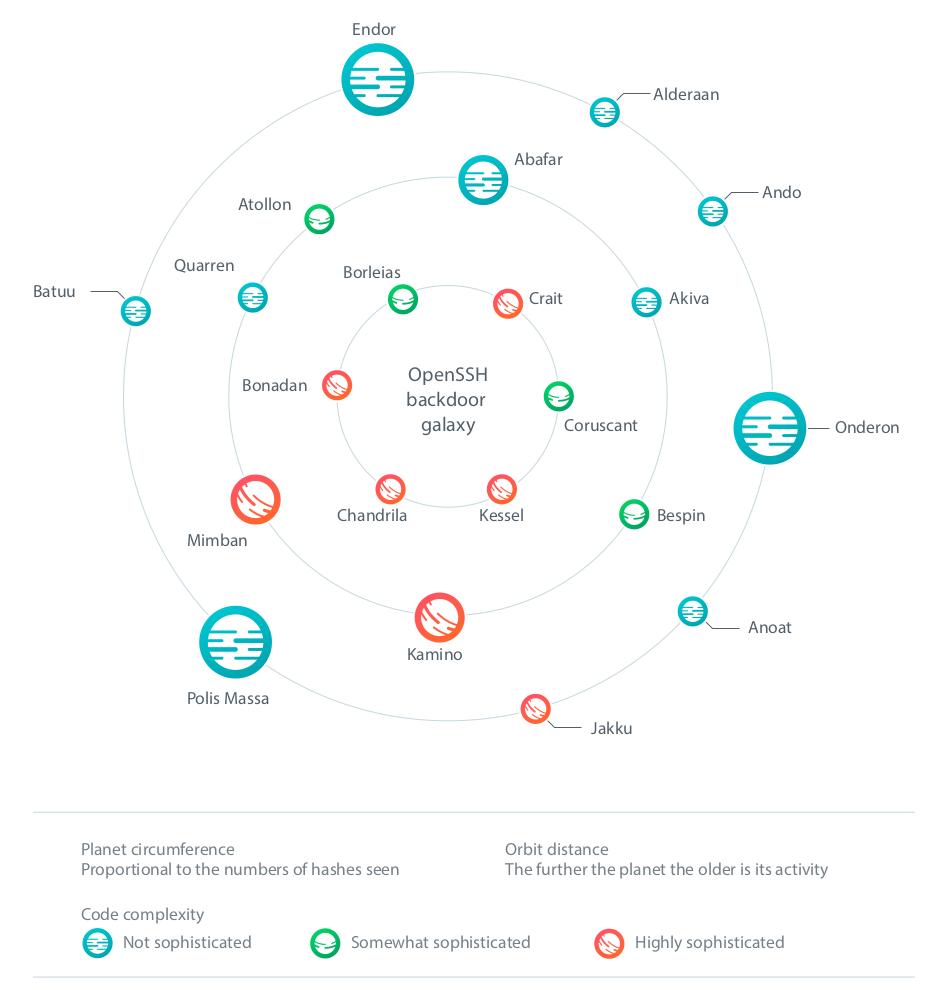
\includegraphics[width=0.55\textwidth]{images/OpenSSH_backdoor_galaxy}
   \captionof{figure}{OpenSSH backdoor families according to ESET research}
   \end{center}

\end{frame}
%%%%%%%%%%%%%%%%%%%%%%%%%%%%%%%%%%%%%%%%%%%%%%%%%%%%%%%%%%%%%%%%%%%%%%%%%%%%%%%


%%%%%%%%%%%%%%%%%%%%%%%%%%%%%%%%%%%%%%%%%%%%%%%%%%%%%%%%%%%%%%%%%%%%%%%%%%%%%%%
\begin{frame}
	\frametitle{OpenSSH backdoors summary (1/2)}
	
   \begin{center}    
   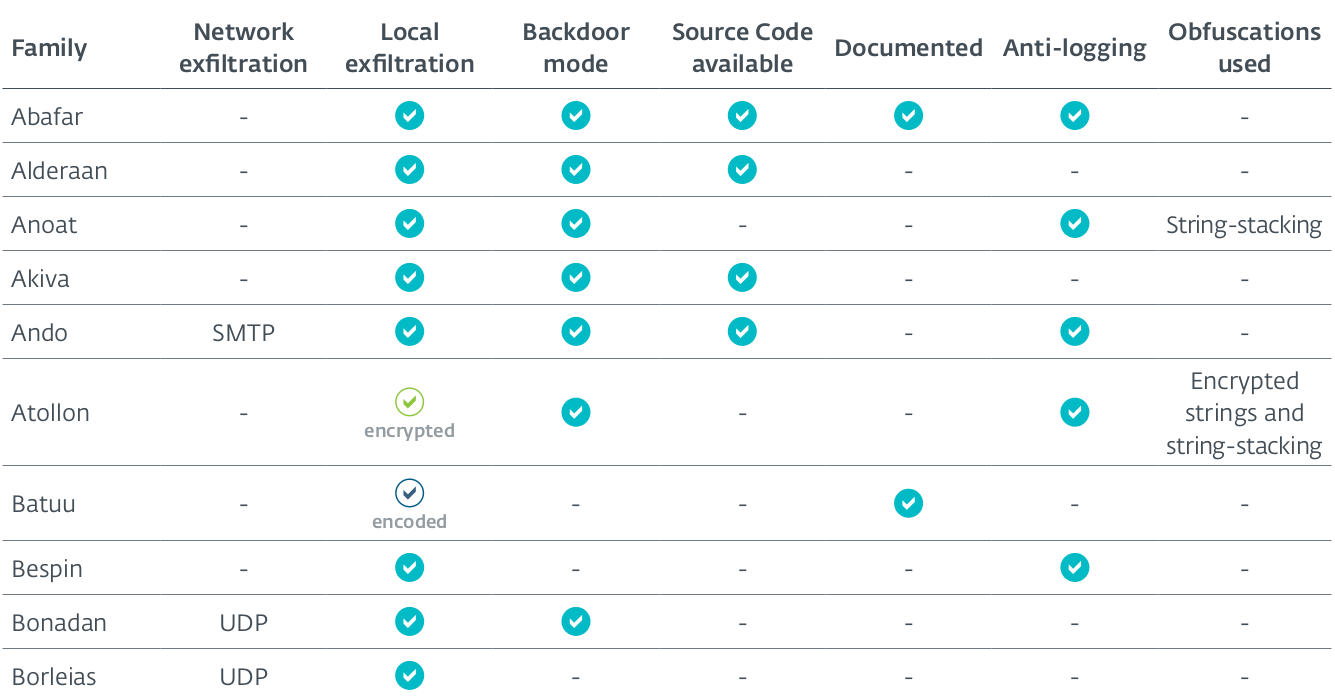
\includegraphics[width=0.85\textwidth]{images/families1}
   \end{center}

\end{frame}
%%%%%%%%%%%%%%%%%%%%%%%%%%%%%%%%%%%%%%%%%%%%%%%%%%%%%%%%%%%%%%%%%%%%%%%%%%%%%%%


%%%%%%%%%%%%%%%%%%%%%%%%%%%%%%%%%%%%%%%%%%%%%%%%%%%%%%%%%%%%%%%%%%%%%%%%%%%%%%%
\begin{frame}
	\frametitle{OpenSSH backdoors summary (2/2)}
	
   \begin{center}    
   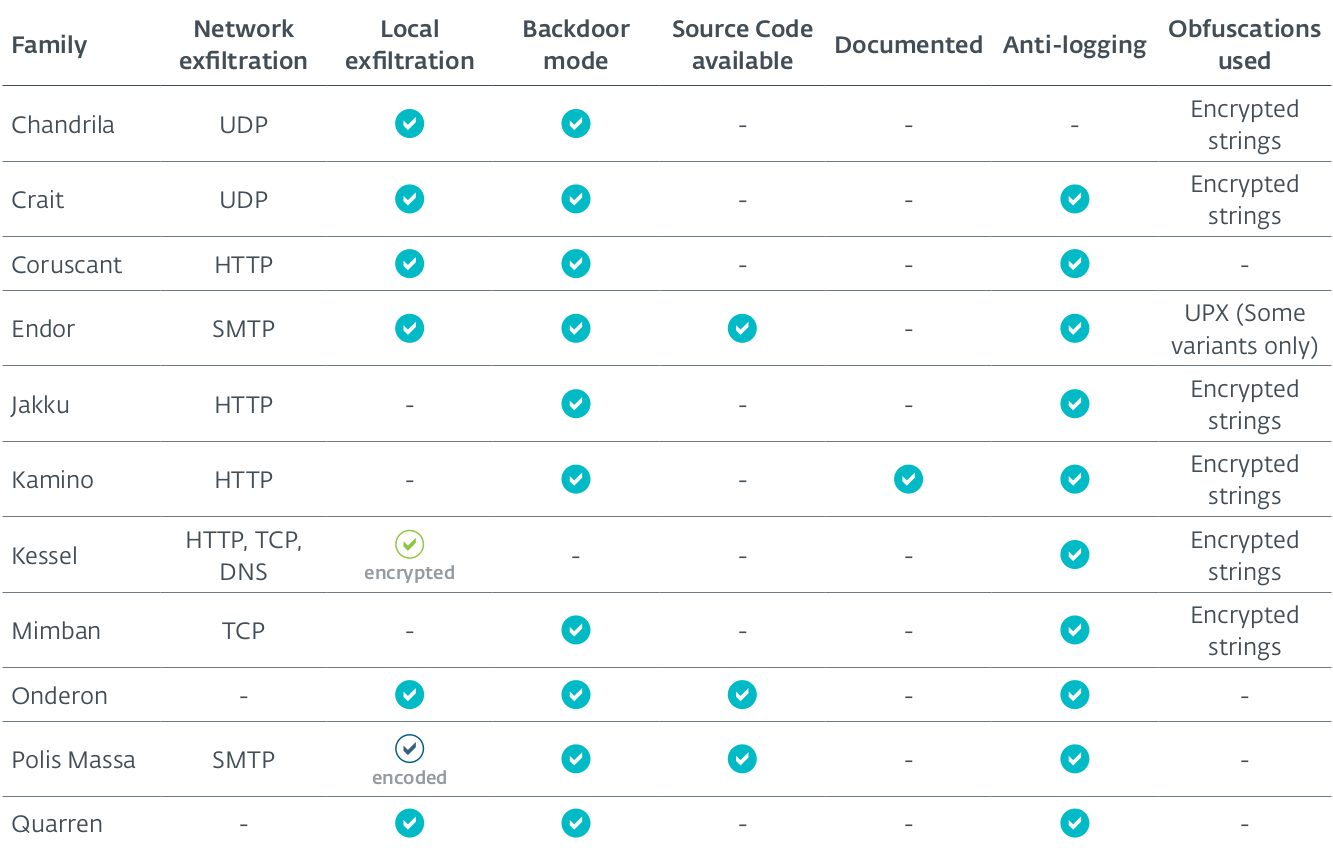
\includegraphics[width=0.85\textwidth]{images/families2}
   \end{center}

\end{frame}
%%%%%%%%%%%%%%%%%%%%%%%%%%%%%%%%%%%%%%%%%%%%%%%%%%%%%%%%%%%%%%%%%%%%%%%%%%%%%%%


%%%%%%%%%%%%%%%%%%%%%%%%%%%%%%%%%%%%%%%%%%%%%%%%%%%%%%%%%%%%%%%%%%%%%%%%%%%%%%%
\begin{frame}
	\frametitle{Chandrila}
	
	Save authentication method, username and password base64-encoded.
	
	\bigskip
	
	Exfiltration of credentials via local file or sent via UDP to a C\&C server.
	
	\bigskip
	
	Distinctive feature: \textbf{can receive commands through the SSH password}.\\
	Two passwords are hardcoded in the backdoor: one to login in the server and another to execute commands, by appending data to the password.
	
	\medskip
	
	In particular:
	
	\smallskip
	
	\textbf{C0011455OpenSSHd} backdoor password for command line.
	\textbf{C001145SOpenSSHd\$\{CMD\}} execute CMD on server.

	\bigskip

  Powerful backdoor mode as attacker can execute command without a shell.
  
\end{frame}
%%%%%%%%%%%%%%%%%%%%%%%%%%%%%%%%%%%%%%%%%%%%%%%%%%%%%%%%%%%%%%%%%%%%%%%%%%%%%%%


%%%%%%%%%%%%%%%%%%%%%%%%%%%%%%%%%%%%%%%%%%%%%%%%%%%%%%%%%%%%%%%%%%%%%%%%%%%%%%%
\begin{frame}
	\frametitle{Bonadan}
	
	Backdoor fork a new thread inside the main function: this thread periodically calls two functions and pause for five minutes.
	
	\bigskip
	
	First function check if there is any \textbf{cryptocurrency miner} installed on the system and removes it.
	
	\bigskip
	
  Second function connect to the C\&C server and send several information about the host over UDP (such as current username, OS version, external IP address, CPU and RAM models, speed of the miner).
  
	\bigskip
	
	Backdoor receive an answer from the C\&C server that can containing a specific command like: create a shell, execute a command on machine, updates the configuration, launch a cryptocurrency mining module.
	
	\bigskip
	
  The backdoor mines the \textbf{Monero cryptocurrency} as part of a mining pool.

	\bigskip
	
  Problem: need to store wallet information inside the server.
  
\end{frame}
	
%%%%%%%%%%%%%%%%%%%%%%%%%%%%%%%%%%%%%%%%%%%%%%%%%%%%%%%%%%%%%%%%%%%%%%%%%%%%%%%


%%%%%%%%%%%%%%%%%%%%%%%%%%%%%%%%%%%%%%%%%%%%%%%%%%%%%%%%%%%%%%%%%%%%%%%%%%%%%%%
\begin{frame}
	\frametitle{Kessel}
	
	\small
	
	Most advanced and recent between all the families. This backdoor includes two main features: a bot functionality and credentials stealing.
	
	\medskip
	
	\textbf{Bot feature}: a bot is launched at the beginning of the OpenSSH main function, generate an ID based on MAC address, collect system information then starts two threads.
  
	\smallskip

  First thread periodically send encrypted information to a C\&C server and eventually create a reverse shell with a specified machine. Second thread repeatedly queries a TXT records in a custom DNS server to get commands.    
  
	\medskip
	
	\textbf{Credential stealing}: reimplements two malicious functions in SSH daemon (\textsc{ssh\_login} and \textsc{user\_auth\_pubkey}) to steal remote host/username, password and local username (or private/public key). Exfiltrate stolen credentials using HTTP, TCP or DNS protocol.
  
   \begin{center}    
   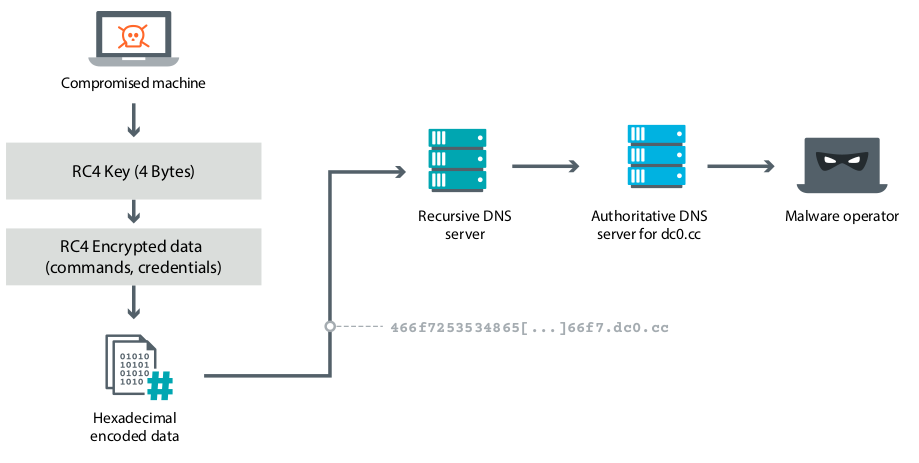
\includegraphics[width=0.45\textwidth]{images/dns_exfiltration}
   \captionof{figure}{DNS exfiltration schema}
   \end{center}

  	
\end{frame}
%%%%%%%%%%%%%%%%%%%%%%%%%%%%%%%%%%%%%%%%%%%%%%%%%%%%%%%%%%%%%%%%%%%%%%%%%%%%%%%


%%%%%%%%%%%%%%%%%%%%%%%%%%%%%%%%%%%%%%%%%%%%%%%%%%%%%%%%%%%%%%%%%%%%%%%%%%%%%%%
\begin{frame}
	\frametitle{Kamino}
	
	First variant of this backdoor already seen in 2013 (as documented in \textbf{[3]}).
	
	\medskip
	
	Used together with an Apache module called DarkLeech to redirect internet traffic.
	
	\medskip
	
	After few years the same backdoor was used again to attack Russian Banks by a group known as Carbanak, resulting in \textbf{$\sim$900 million dollars}. 
	
	
   \begin{center}    
   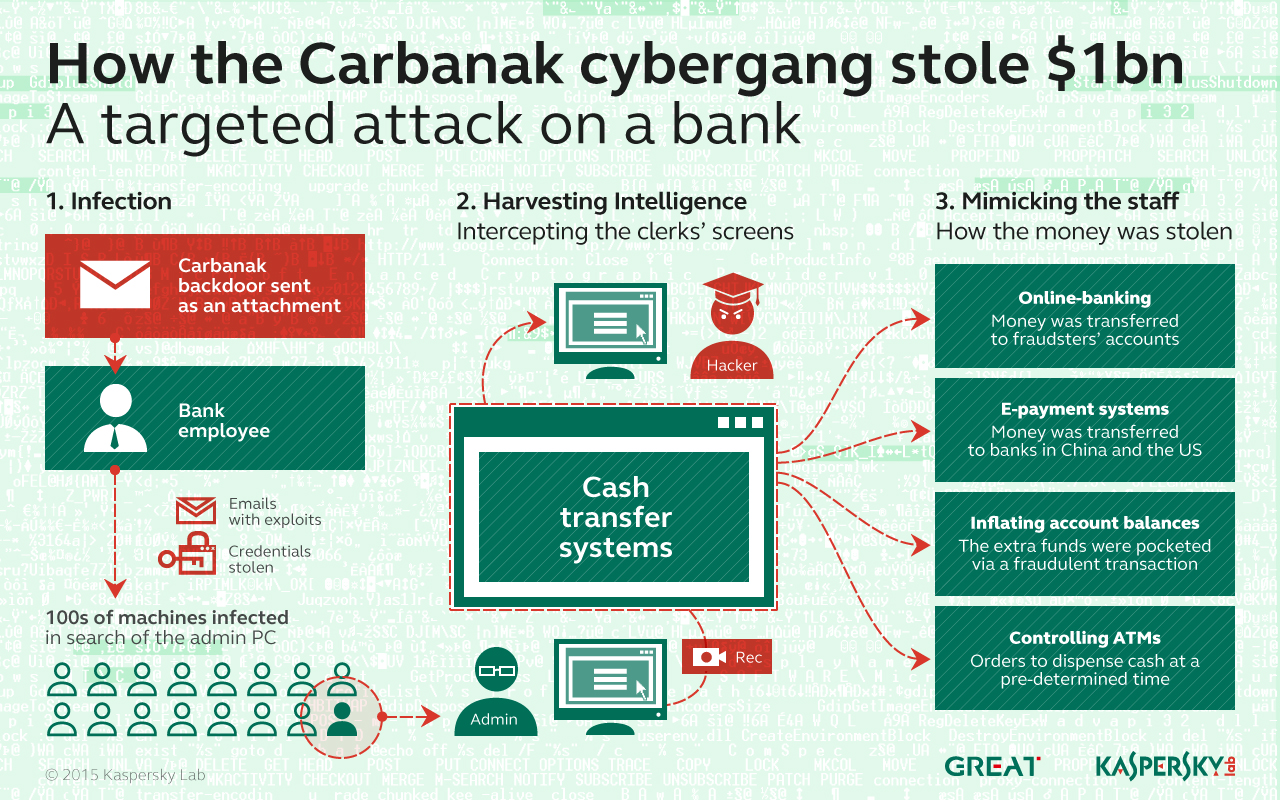
\includegraphics[width=0.55\textwidth]{images/Carbanak}
   \captionof{figure}{Carbanak attack (source: Kaspersky\textbf{$^{[7]}$})}
   \end{center}

\end{frame}
%%%%%%%%%%%%%%%%%%%%%%%%%%%%%%%%%%%%%%%%%%%%%%%%%%%%%%%%%%%%%%%%%%%%%%%%%%%%%%%
